% !TEX TS-program = pdflatex
% !TEX encoding = UTF-8 Unicode

% This is a simple template for a LaTeX document using the "article" class.
% See "book", "report", "letter" for other types of document.

\documentclass[11pt]{article} % use larger type; default would be 10pt

\usepackage[utf8]{inputenc} % set input encoding (not needed with XeLaTeX)
%\usepackage{babel}
%%% Examples of Article customizations
% These packages are optional, depending whether you want the features they provide.
% See the LaTeX Companion or other references for full information.

%%% PAGE DIMENSIONS
\usepackage{geometry} % to change the page dimensions
\geometry{a4paper} % or letterpaper (US) or a5paper or....
% \geometry{margin=2in} % for example, change the margins to 2 inches all round
% \geometry{landscape} % set up the page for landscape
%   read geometry.pdf for detailed page layout information

\usepackage{graphicx} % support the \includegraphics command and options

% \usepackage[parfill]{parskip} % Activate to begin paragraphs with an empty line rather than an indent

%%% PACKAGES
\usepackage{booktabs} % for much better looking tables
\usepackage{array} % for better arrays (eg matrices) in maths
\usepackage{paralist} % very flexible & customisable lists (eg. enumerate/itemize, etc.)
\usepackage{verbatim} % adds environment for commenting out blocks of text & for better verbatim
\usepackage{subfig} % make it possible to include more than one captioned figure/table in a single float
\usepackage{setspace} %paquete para interlineado
\usepackage{graphicx} %para insertar graficos
\usepackage{parskip} % npi de q es
\usepackage{color} %colores
\usepackage{float}


% These packages are all incorporated in the memoir class to one degree or another...

%%% HEADERS & FOOTERS
\usepackage{fancyhdr} % This should be set AFTER setting up the page geometry
\pagestyle{fancy} % options: empty , plain , fancy
\renewcommand{\headrulewidth}{0pt} % customise the layout...
\lhead{}\chead{}\rhead{}
\lfoot{}\cfoot{\thepage}\rfoot{}

%%% SECTION TITLE APPEARANCE
\usepackage{sectsty}
\allsectionsfont{\sffamily\mdseries\upshape} % (See the fntguide.pdf for font help)
% (This matches ConTeXt defaults)

%%% ToC (table of contents) APPEARANCE
\usepackage[nottoc,notlof,notlot]{tocbibind} % Put the bibliography in the ToC
\usepackage[titles,subfigure]{tocloft} % Alter the style of the Table of Contents
\renewcommand{\cftsecfont}{\rmfamily\mdseries\upshape}
\renewcommand{\cftsecpagefont}{\rmfamily\mdseries\upshape} % No bold!

%%% END Article customizations

\usepackage[spanish]{babel}
\usepackage{listings} 
%%% The "real" document content comes below...

\title{Proyecto de Lenguajes de Programaci\'on \\ Primer Parcial}
\author{\\Fausto Mora \\Christian Vergara \\ Angel Gonz\'alez}
%\date{} % Activate to display a given date or no date (if empty),
         % otherwise the current date is printed 
\begin{document}


%\date{} % Activate to display a given date or no date (if empty),
         % otherwise the current date is printed 

\maketitle

\newpage
\thispagestyle{empty}
\tableofcontents

\newpage
\thispagestyle{empty}


\section{\textbf{Introducción}}

Este documento describe la realizaci\'on de un proyecto en la plataforma Android. El proyecto consiste en la elaboraci\'on de una aplicaci\'on para dispositivos m\'oviles y a su vez corresponde al cl\'asico juego Buscaminas que se hiz\'o popular en el sistema Windows. La aplicaci\'on es fiel al juego original y mantiene su jugabilidad tradicional.
\\El proyecto fue realizado como proyecto de primer parcial para la materia de Lenguajes de Programaci\'on con el fin de cubrir los siguientes puntos de interes:
\begin{itemize}
\item Conocer la sintaxis y semántica de otro lenguaje de programación.
\item Escribir un programa utilizando un lenguaje de diferente paradigma y que nos permita comparar sus características y similitudes con otros lenguajes ya conocidos.
\item Fomentar el uso de herramientas colaborativas para la elaboraci\'on de proyectos.
\item Realizar una aplicaci\'on para dispositivos m\'oviles de la plataforma Android.
\end{itemize}
Para concluir en la realizaci\'on del proyecto formamos un grupo de tres personas y empezamos a desarrollarlo de manera conjunta para implementar las caracter\'isticas de la aplicaci\'on. Como recursos para aprender la sintaxis y sem\'antica del lenguaje de programaci\'on para la plataforma en Android consultamos distintas fuentes en l\'inea. Como herramienta de versionamiento de proyectos utilizamos GitHub. Esto nos permiti\'o trabajar de manera remota desde donde lo deseabamos y poder revisar los avances de cada integrante en l\'inea. Ocasionalmente tuvimos que reunirnos para discutir el rumbo del proyecto e implementar caracter\'isticas que requerieron nuestro esfuerzo conjunto.
\\Este documento presenta de manera organizada la documentaci\'on de nuestro proyecto incluyendo aspectos como la descripci\'on del proyecto en s\'i donde inclu\'imos los objetivos generales y espec\'ificos que busca cumplir nuestra aplicaci\'on, el alcance del mismo donde describimos las caracter\'isticas que logramos implementar y las que no, diagrama de casos de uso y de clases implementadas en el proyecto, conclusiones elaboradas en base a nuestra experiencia obtenida al realizar la aplicaci\'on, y finalmente una secci\'on de anexos donde incluimos un manual de nuestra aplicaci\'on.

\section{\textbf{Descripci\'on del Proyecto}}
\subsection{\textbf{Prop\'osito}}
Al finalizar el proyecto, los responsables del mismo presentaremos una aplicaci\'on para dispositivos m\'oviles para la plataforma Android; desarrollado haciendo uso del entorno de desarrollo Eclipse, y de herramientas de software y dispositivos en donde pueda ser emulado y ejecutado, a fin de adquirir conocimientos en dicho lenguaje de programaci\'on y las herramientas involucradas, para fortalecer nuestras competencias en el "Desarrollo de proyectos con diferentes lenguajes de programaci\'on representando diferentes paradigmas de lenguajes."
\subsection{\textbf{Producto}}
La aplicaci\'on desarrollada corresponde al juego \textsl{Buscaminas} del sistema Windows. El juego será ejecutable en distintos dispositivos que soporten el sistema Andorid, teniendo preferencia en los dispositivos m\'oviles de pantalla grande ( para un mejor uso de la aplicaci\'on).
\\El producto ser\'a desarrollado en el entorno Eclipse disponiendo del SDK para Android. El juego ser\'a emulado en el software haciendo uso del software Genymotion as\'i como del mismo emulador que nos provee Eclipse y podr\'a ser ejecutado en dispositivos Android con un API desde la versi\'on 2.1 (Dependiendo de la disponibilidad de componentes presentes en dicho API y que sean usados en nuestro proyecto), hasta las versiones de Andorid m\'as recientes.
\subsection{\textbf{Objetivos}}
Para lograr cumplir nuestro prop\'osito planteamos los siguientes objetivos.
\subsubsection{\textbf{Objetivos Generales}}
\begin{itemize}
\item Desarrollar una Aplicaci\'on para el sistema Android.
\item Conocer la sintaxis y sem\'antica del lenguaje de programaci\'on de la platarforma Android.
\item Desarrollar competencias en la utilizaci\'on de diferentes paradigmas de los lenguajes de programaci\'on.
\end{itemize}
\subsubsection{\textbf{Objetivos Espec\'ificos}}
\begin{itemize}
\item Implementar el juego Buscaminas del sistema Windows respetando todas sus funcionalidades.
\item Hacer uso de herramientas que nos permitan desarrollar aplicaciones para dispositivos m\'oviles.
\item Utilizar las caracter\'isticas del lenguaje de programac\'on Android de manera eficiente y \'optima.
\end{itemize}
\subsection{\textbf{Alcance}}
\subsubsection{\textbf{Caracter\' isticas implementadas}}
El \'area para la que esta desarrollado nuestro proyecto es la de dispositivos m\'oviles.
La aplicaci\'on desarrollada posee caracter\'isticas muy similares al juego Buscaminas de Windows y a continuaci\'on se mencionan las caracter\'isticas implementadas en en plazo de realizaci\'on del proyecto.
\\La aplicaci\'on consta de una pantalla principal  donde se presenta al usuario las siguientes opciones: Iniciar Juego, Instrucciones, Ranking, Desarrolladores y Salir. Cada opci\'on presentada en la pantalla principal desencadena una actividad diferente al ser seleccionada.
\\Para Iniciar el juego hay que escoger entre las tres dificultades disponibles o la opci\'on Personalizado. Las tres dificultades implementadas son: Principiante, Normal, Experto. En la primera se presenta un tablero de juego de 8 x 8 celdas donde se hallan escondidas 10 minas. En la segunda se presenta un tablero de juego de 16 x 16 celdas donde se hallan escondidas 40 minas. En la tercera se presenta un tablero de juego de 16 x 30 celdas donde se hallan escondidas 99 minas. La opci\'on de juego personalizado le permite al usuario determinar las dimensiones del tablero (n\'umero de celdas por columna y por fila) asi como el n\'umero de minas escondidas en el tablero.
\\Se implemento la manera de asignar minas en el tablero una vez que se haya dado el primer clic en una de las casillas. Esto se realizo\' o con el fin de evitar que el usuario pierda una partida con el primer clic.
\\En la pantalla de juego se incluye un reloj que muestra segundo a segundo el tiempo que transcurre durante el juego. Este reloj inicia su marcha desde el primer clic.
\\Tambi\'en se implemeto un bot\' on de reinicio que permite empezar un nuevo juego en cuanto es presionado. Puede ser usado en cualquier momento. Este es un bot\'on animado.
\\Para poder guardar las puntuaciones m\' as sobresalientes que los usuarios logren se hace uso de una base de datos para Android (SQLite). Aqu\' i se almacenan los nombres y puntuaciones de los usuarios que logren ingresar en el ranking. El Ranking solo estar\'a formado  conformado por puntajes logrados en las dificultades: Principiante, Normal y Experto.
\\La aplicaci\'on inicia con pantalla principal vertical, una vez iniciado el juego la rotaci\'on del dispositivo se bloquea y solo puede ser usado de manera horizontal.

\subsubsection{\textbf{Caracter\' isticas no implementadas}}

No se implemento el uso de la bandera.

\subsubsection{\textbf{Caracter\' isticas extras}}

Se implemento un algoritmo que cambia el color de los numeros que advierten de minas en las cercan\'ias en cada click o click largo.

\subsection{\textbf{Entregables}}
El proyecto incluye la entrega de lo siguiente:

\begin{itemize}
\item El link del repositorio GIT donde se encuentra el c\'odigo fuente.
\item Documentación en LaTeX ( incluidos el PDF y el c\'odigo fuente). Estos documentos y todos los recursos que se necesiten para la ejecuci\'on del c\'odigo fuente deber estar dentro de una carpeta llamada \textsl{doc}.
\item  El proyecto ser\'a presentado en un dispositivo m\'ovil corriendo con todas sus funcionalidades.
\end{itemize}

\subsection{\textbf{Restricciones}}
La principal limitaci\'on de nuestro proyecto se debe al tama\~no de la pantalla del dispositivo en donde se ejecute.
Esto se debe al dise\~no del tablero del juego. Al estar compuesto de celdas y al ser una aplicaci\'on t\'actil se dificulta la jugabilidad en dispositivos de pantalla peque\~na.
Es por esta raz\'on que es preferible ejecutar la aplicaci\'on en dispositivos de pantalla grande. Sin embargo, esta restricci\'on es solo visual, mas no afecta a la funcionalidad de la aplicac\'on, es decir, que la aplicaci\'on puede ser normalmente ejecutad y probada en cualquier dispositivo independientemente del tama\~no de su pantalla.

\newpage
\thispagestyle{empty}

\section{\textbf{Diagramas de casos de uso }}

\begin{center}

	\begin{figure}[h!]
  		\centering
    		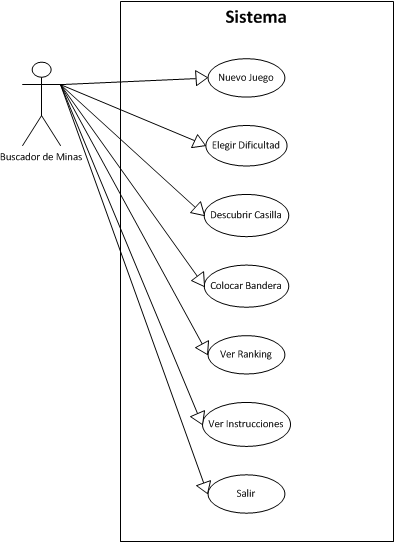
\includegraphics[width=0.7\textwidth]{imagenes/casosdeusos.png}
  		\caption{Casos de Usos}
		\label{fig:casosdeusos}
	\end{figure}
\end{center}

\newpage
\thispagestyle{empty}

\section{\textbf{Diagrama de clases }}

\begin{center}

	\begin{figure}[h!]
  		\centering
    		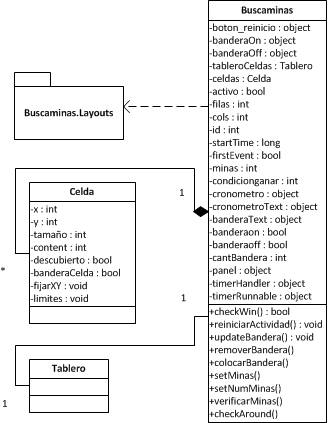
\includegraphics[width=0.7\textwidth]{imagenes/diagramaClases.jpg}
  		\caption{Diagrama de Clases}
		\label{fig:diagclases}
	\end{figure}
\end{center}

\newpage
\thispagestyle{empty}

\section{\textbf{Conclusiones}}

Observamos que Android es un lenguaje que nos presta muchas opciones al momento de programar. Android nos permite programar de distintas maneras y nos da muchas herramientas para lograr que nuestras aplicaciones sean lo m\'as personalizadas posibles.
\\Aunque se trata de un lenguaje nuevo para nosotros no lo era en su totalidad ya que es muy similar a Java lo cual permiti\'o que el proceso de aprendizaje sea relativamente lento y muy amigable. Observamos tambi\'en que trabajar en Android es m\'as ordenado que trabajar en otros lenguajes ya que el uso de ficheros XML nos facilita entender como esta estructurado el c\'odigo.
\\Logramos implementar el juego Buscaminas casi en su totalidad. La \'unica funci\'on no implementada fue la de agregar banderas. Lamentablemente, cuando decidimos implementarlas de las tres maneras que sabiamos que era posible tuvimos muchos problemas con respecto a la funcionalidad principal del juego. Las tres formas por las que consideramos posible hacerlo y por las que intentamos cumplir con esta funcionalidad son: Drag and Drop, uso de Botones y uso de Clicks prolongados.
\\Muchas de las heramienta que Android nos presta fueron cruciales para ciertas funcionalidades de la aplicaci\'on. Por ejemplo, para implementar la parte del Ranking teniamos m\'ultiples opciones, de entre las cuales optamos por el uso de un motor de base de datos incluido en el mismo sistema. Este es SQLite el cual nos permitio hacer que implementar esta funcionalidad sea relativamente sencillo.
\\Aunque con un poco de problemas, logramos emular exitosamente la mayor\'ia de las pruebas. Los problemas que mencionamos se tratan sobre el tiempo que cuesta emular un dispositivo Android en una computadora. Tuvimos que tratar de asegurarnos con revisiones exhaustivas que un c\'odigo que queirmos probar tenga la menor cantidad de errores de funcionalidad posibles para ahorrar tiempo. La herramienta Genymotion presento los mismos problemas que la que nos proporcionaba Eclipse por lo que la mayor\'ia de veces usamos la \'ultima.
\\Gracias al soporte que presta el SDK de Android para que nuestra aplicaci\'on sea ejecutable en gran variedad de API's pudimos lograr las pruebas en dispositivos sin problema alguno. Disponiamos de dispositivos m\'oviles Android de diferentes API's y resoluciones y no experimentamos problemas que tengan que ver con sus caracter\'isticas durante las pruebas.


\newpage
\thispagestyle{empty}

\section{\textbf{Anexos}}
\subsection{\textbf{Manual de la Aplicaci\' on}}
\subsubsection{\textbf{Pantalla Principal}}
Esta es la primera pantalla que presenta la aplicaci\' on al iniciarse. En ella estan los botones que el usuario puede seleccionar para iniciar una actividad.
\begin{center}

	\begin{figure}[h!]
  		\centering
    		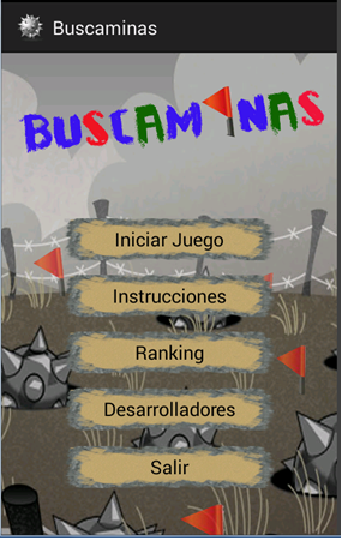
\includegraphics[width=0.4\textwidth]{imagenes/PantallaPrincipal.PNG}
  		\caption{Pantalla Principal de la Aplicaci\' on}
		\label{fig:pantallaprincipal}
	\end{figure}
\end{center}

Para concocer las instucciones el usuario debe hacer clic en el bot\'on Instrucciones. A continuaci\'on se presentara una pantalla con las instrucciones del juego.
\begin{center}

	\begin{figure}[h!]
  		\centering
    		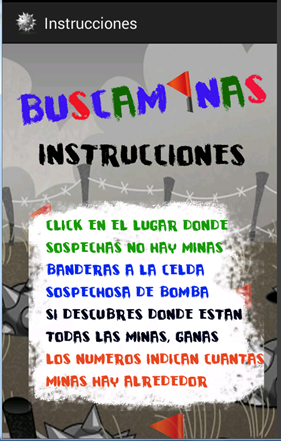
\includegraphics[width=0.3\textwidth]{imagenes/Instrucciones.PNG}
  		\caption{Pantalla con las Instrucciones del juego}
		\label{fig:instrucciones}
	\end{figure}
\end{center}

\newpage
\thispagestyle{empty}

Para consultar las m\'as altas puntuaciones obtenidas por los usuarios del juego se debe seleccionar la opci\'on Ranking. A contiuaci\'on se presentara una pantalla con las puntuaciones m\'as altas clasificadas seg\'un la dificultad.
\begin{center}

	\begin{figure}[h!]
  		\centering
    		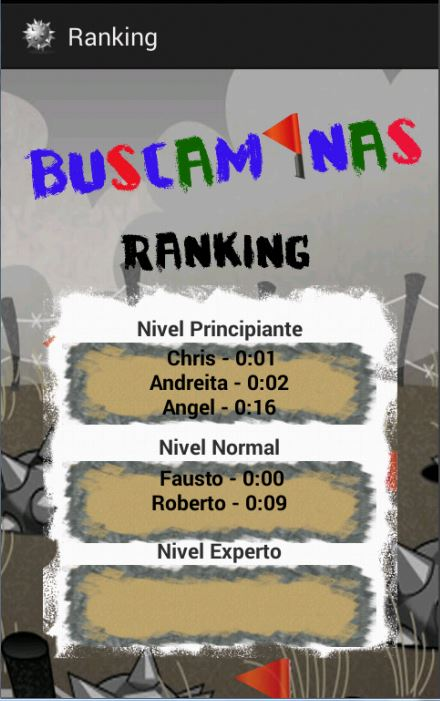
\includegraphics[width=0.3\textwidth]{imagenes/Ranking.JPG}
  		\caption{Pantalla que contiene las puntuaciones  m\'as sobresalientes de los usuarios}
		\label{fig:ranking}
	\end{figure}
\end{center}

\newpage
\thispagestyle{empty}

En la opci\'on Desarrolladores el usuario puede obtener informaci\'on acerca de los desarrolladores del juego. A continuaci\'on se presentara una pantalla con esta informaci\'on.
\begin{center}

	\begin{figure}[h!]
  		\centering
    		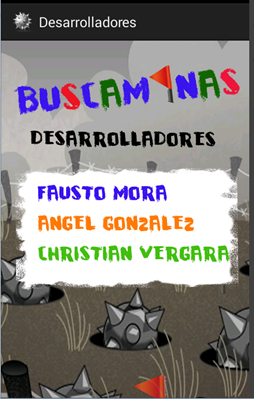
\includegraphics[width=0.3\textwidth]{imagenes/Desarrolladores.PNG}
  		\caption{Pantalla que contiene la informaci\'on de los desarrolladores del juego}
		\label{fig:desarrolladores}
	\end{figure}
\end{center}
La opci\'on Salir le permite al usuario abandonar el juego. Cierra por completo la aplicaci\'on.
\\Para comenzar a jugar, el usuario debe escoger la Opci\'on Iniciar Juego. Luego se desplegar\'a una pantalla donde se le solicita al usuario escoger entre 4 dificultades. Estas son: Principiante, Normal, Experto y Personalizado.
\begin{center}

	\begin{figure}[h!]
  		\centering
    		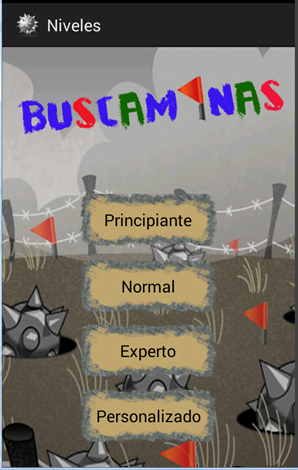
\includegraphics[width=0.25\textwidth]{imagenes/Dificultades.PNG}
  		\caption{Pantalla de selecci\'on de dificultad}
		\label{fig:dificultades}
	\end{figure}
\end{center}

\newpage
\thispagestyle{empty}

\subsubsection{\textbf{Partes de la Pantalla de Juego}}

\begin{center}

	\begin{figure}[h!]
  		\centering
    		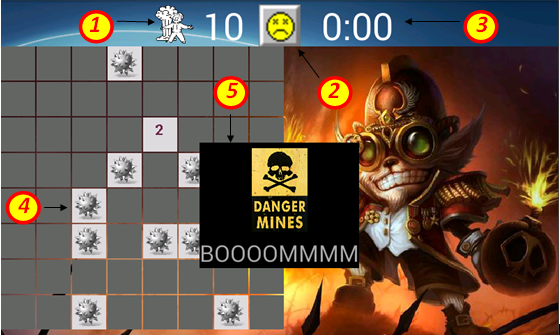
\includegraphics[width=0.5\textwidth]{imagenes/partesdeltablero1.PNG}
  		\caption{Tablero de una partida perdida en dificultad Normal}
		\label{partesdeltablero}
	\end{figure}
\end{center}

La pantalla de juego est\'a formada por un tablero de juego en donde se colocan las minas y un panel con informaci\'on y un bot\'on de reinicio.
\\A continuaci\'on se describen las partes del tablero se\~naladas en la \textbf{Figura \ref{partesdeltablero}}:

\begin{itemize}

\item \textbf{1. Cantidad de minas:} Este panel muestra la cantidad de minas que se encuentran dispersas en el tablero. Consta de una imagen animada que cambia de acuerdo a las acciones del usuario.
\item \textbf{2. Bot\'on Reinicio:} Este bot\'on permite reiniciar el juego. Es un bot\'on animado que cambia dependiendo de las acciones que realize el jugador sobre el tablero. Mientras no haya actividad la cara en el bot\'on se mantiene sonriente. Si se se presiona una celda la cara cambiara a una cara de suspenso. Si la celda donde se presiona no tiene mina la cara vuelve a su estado inicial. Sin embargo, si se encuentra una mina en la celda seleccionada la cara cambiara de estado demostrando que se ha perdido la partida.
\item \textbf{3. Reloj:} El reloj muestra el tiempo que transcurre durante el juego segundo a segundo e inicia su marcha con el primer click sobre el tablero. El tiempo se traduce en el record del jugador. Mientras menos tiempo se tarde el jugador en ganar su puntuaci\'on mejorar\'a.
\item \textbf{4. Minas:} Las minas se dispersan en el tablero al momento de hacer el primer click. Una mina permanece escondida hasta que el jugador descubre una celda que la contenga. Cuando se descubre una celda que conten\'ia una mina se pierde la partida.
\item \textbf{5. Mensajes:} Los mensajes se presentan al final de un juego y pueden ser mensajes de partida perdida o ganada. Los mensajes permanecen temporalmente en pantalla.

\end{itemize}

\subsubsection{\textbf{Dificultades de Juego}}

Las dificultades afectan directamente a las dimensiones del tablero, as\'i como al n\'umero de minas que se reparten en \'el. en todos lo casos la jugabilidad se mantiene. A continuaci\'on se listan las dimensiones y cantidad de minas presentes en los tableros de dificultades ajustadas:

\begin{itemize}
\item La dificultad Principiante presenta un tablero de 8x8 celdas y 10 minas.
\item La dificultad Normal presenta un tablero de 16x16 celdas y 40 minas.
\item La dificultad Principiante presenta un tablero de 16x30 celdas y 99 minas.
\end{itemize}

\begin{center}

	\begin{figure}[h!]
  		\centering
    		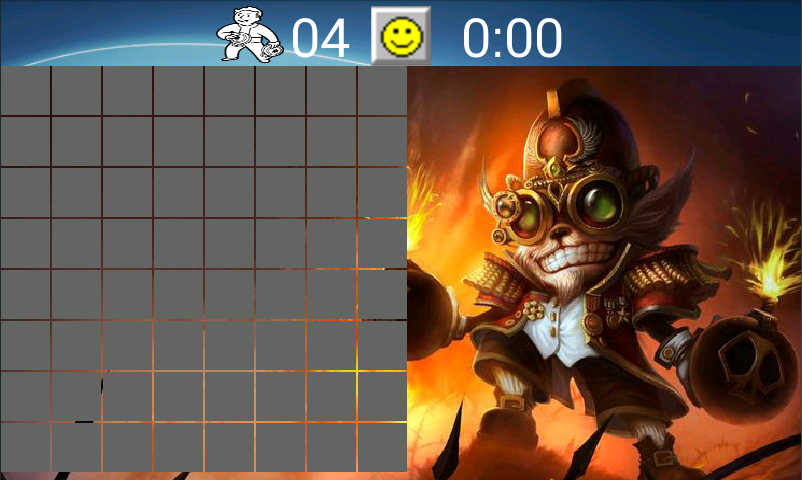
\includegraphics[width=0.35\textwidth]{imagenes/tableroPrincipiante.PNG}
  		\caption{Tablero de dificultad Principiante de 8x8 celdas}
		\label{fig:tableroprincipiante}
	\end{figure}
\end{center} 

\begin{center}

	\begin{figure}[h!]
  		\centering
    		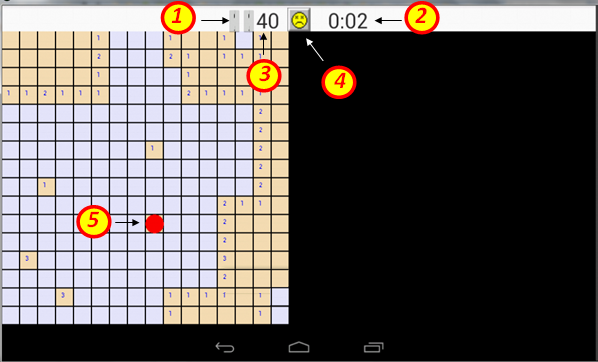
\includegraphics[width=0.35\textwidth]{imagenes/tableroNormal.PNG}
  		\caption{Tablero de dificultad Normal de 16x16 celdas}
		\label{fig:tableronormal}
	\end{figure}
\end{center} 

\begin{center}

	\begin{figure}[h!]
  		\centering
    		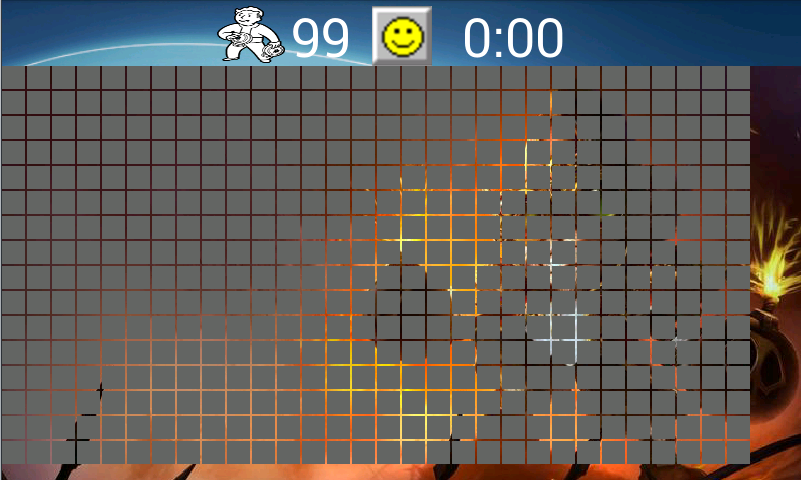
\includegraphics[width=0.35\textwidth]{imagenes/tableroDificil.PNG}
  		\caption{Tablero de dificultad Experto de 16x30 celdas}
		\label{fig:tableroexperto}
	\end{figure}
\end{center} 

El juego Personalizado permite al usuario establecer las dimensiones del tablero y tambi\'en el n\'umero de minas que pueden existir en \'el. El usuario puede escoger como m\'inimo n\'umero de filas o columnas la cantidad de 8, y como m\'aximo la cantidad de 30, es decir, que el m\'inimo tablero que se puede construir en dificultad Personalizado es un tablero de 8x8 y el m\'aximo es de 30x30 celdas. De manera similar, el n\'umero de minas que se pueden colocar en el tablero es mayor a cero y menor al n\'umero de celdas. 

\begin{center}

	\begin{figure}[h!]
  		\centering
    		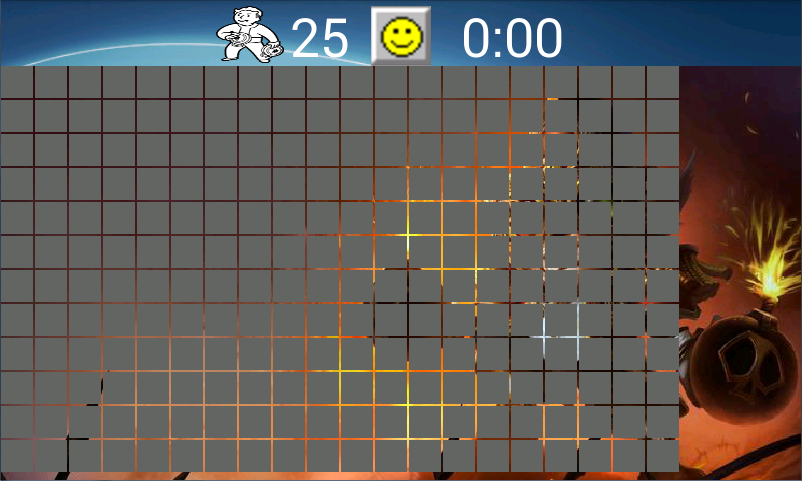
\includegraphics[width=0.3\textwidth]{imagenes/tableroPersonalizado.PNG}
  		\caption{Tablero de dificultad Personalizado de 12x20 celdas}
		\label{fig:tableropersonalizado}
	\end{figure}
\end{center} 



\end{document}
